\chapter[Summary]{Summary}\label{chap:summary}
This thesis analyzed a multitude of aspects that need to be considered when we try to support users in password authentication with persuasive design. Hereby, the following research questions were addressed:

\begin{itemize}
	\item[\textbf{RQ1}] What is the role of psychological factors and mental models for password selection and coping strategies?
	\item[\textbf{RQ2}] How can password authentication be simplified for users? 
	\item[\textbf{RQ3}] How can we design persuasive strategies to support users in any password-related tasks?
\end{itemize}

Since password authentication has been under investigation for several decades, we first delimited the landscape of related work in Part \ref{part:related_work}. This helped us partially answer all three research questions and identify open questions that had still been underexplored (see Chapter \ref{chap:rw:summary}). In Parts \ref{part:problem_space} and \ref{part:design_space}, we reported on a number of empirical experiments and explorative research studies to investigate both human factors and environmental constraints of password authentication. \textit{RQ1} was mainly investigated with online studies in the wild and with survey methods. We explored the mental models of password strength by innovating a research method to inexpensively collect data in the wild. Moreover, we conducted multiple surveys to explore associations between personality and attitudes and behaviors in authentication. We tried to answer \textit{RQ2} with mixed methods, both on the qualitative and the quantitative side. Here, we explored the needs users have in persuasive feedback with a survey and participatory design approach, and derived a solution based on the Decoy effect and emojis inside text-based passwords. Finally, to answer \textit{RQ3}, we discussed a framework to guide the design of persuasive strategies in Chapter \ref{chap:perdespassup}, which we then also applied to create a novel password-manager. The following sections discuss the central insights and show how they are connected.

\section{Central Contributions and Insights}
\subsubsection{Psychological Factors and Mental Models in Authentication}
% related work mostly _describes_ behaviors and coping strategies, but not the mental models behind them.
% real world password authentication often sees it as a small hurdle, but not worthy of in-depth ux design.
In Chapter \ref{chap:rw:user_perspective}, we found that most related work \textit{describes} coping strategies. Only sometimes the contributing factors like educational background, psychographics, or mental models that foster certain coping strategies are addressed. %Few password alternatives, as presented in Chapter \ref{chap:rw:passwords}, are mature enough to allow investigation of human factors outside the lab, and there is even less insight into the mental models involved. 
%At the same time, real-world authentication systems also often neglects such human factors, which aggravates security issues.

% PASDJO
We filled this gap in several ways. First, we investigated the mental models of password strength, because these are believed to be highly influential on actual password choice. For these purposes, we innovated on research methods to understand latent password strength perceptions: \textit{PASDJO}, the password game, helped in showing that passphrases are often underestimated by users, although \gls{NIST} has started to propagate them in favor of highly complex passwords (see Chapter \ref{chap:pasdjo}). The long-standing belief that strong passwords must include a wide range of characters was clearly visible in the data collected during one year of public deployment. However, users were by and large capable of judging the quality of passwords. This constitutes evidence that users are most likely aware of their actions when they  select strong and weak passwords for different purposes. This gives rise to a shift in the way we support users in password selection: In many cases it is unnecessary to provide feedback on strength, because users can estimate it well. Therefore, we can tackle other risky behaviors. 
% Policy Audit
In fact, password strength is often a secondary risk factor, if users reuse passwords too carelessly. To investigate the real-world constraints for password reuse, we audited the composition policies of the 83 most visited web-sites in Germany (see Chapter \ref{chap:policies_reuse}). We were able to show that it is easy for users to reuse a single password on most sites: it only has to be nine or ten characters long and consist of lower- and uppercase letters and digits. Hence, this finding is another indication that password policies have shaped the mental model that at least three different character classes are absolutely required to form a strong password -- and that reuse is less critical, because it is not prevented. Moreover, users do not need a password manager if their go-to passwords have these features. However, as soon as they add symbols in the belief that this fosters password strength even more, the success rate to reuse this password drops significantly. So, in that case, rejecting passwords based on certain symbols might leave users wondering why these do not boost password strength. The result is a cognitive dissonance in the users' mental models. To resolve this, websites could provide some kind of explanation as to their policy choice, but most fail to do this. Besides, it is very unlikely that they disallow certain symbols hamper password reuse. As a take-away, service providers need to start accepting Unicode passwords without arbitrary length restrictions to avoid confusing users. This allows automatically generating unique passwords of all kinds, which can drive the adoption of password managers. At the same time, Unicode passwords have more ramifications on the use of emojis, which we discuss below. 
% and, if necessary, random password generators, which are the only line of defense for users in mitigating offline attacks \cite{Florencio2016CommACM}. At the same time, 
%1) find ways to detect overly re-used passwords and 2) 

% PERSONALITY
Real-world constraints like composition policies thus shape mental models and coping strategies. On the other hand, there is a spectrum of password coping strategies that cannot be explained by environmental factors alone. We hypothesized that a user's personality might play a role in password selection and coping behavior. In three studies (see Chapter \ref{chap:pws_and_personality}), we examined how personality might be associated with different password tasks. We found that personality was a weak, but non-negligible factor in predicting how different user groups deal with policies, perceive strength, or choose passwords. The data allowed us to create user segments in the form of personas that can be used in the development of authentication schemes and support strategies. 
% PWMs
As a side effect, we observed that people with a background in an IT-related field were more likely to adopt a password manager. Looking at the generally low adoption rates of such software, we explored how users perceive password managers in Chapter \ref{chap:mental_models_pwm}. We contributed the notion that users appreciate this kind of tool once they were first exposed to the technology, e.g. at work. If they had never used a password manager before, they were unable to anticipate how it might help them. We distinguished separate spaces that shape mental models about password managers, however, these were currently not fully matched by commercial software. Consequently, there are novel opportunities to re-design password-managers to better support users. 

% summary
In summary, we have to understand different dimensions of factors that contribute to mental models. Environmental constraints like password policies probably have the largest influence. Much traditional advice on how to form ``good passwords'' has led to a skewed mental model of password strength. Second, professional and educational factors are associated in how well users deal with password tasks. Finally, personality also contributes to the shaping of mental models, and warrants further research in this direction. %Current user interfaces, e.g. web sites, do not seem to take mental models into account when they try to simplify the task. 

\subsubsection{Simplification Strategies}
% state of the world
Having explored mental models and other psychological factors in password authentication, we noted that users do not always correctly make sense of authentication user interfaces. To simplify tasks, researchers have tried numerous approaches. Most notably, strength feedback in the form of password meters and real-time feedback about policy fulfillment have been seen as the state-of-the-art to simplify password selection. These solutions generally assume that there is a policy in place and users struggle to meet it, which is the case in many situations.
% user need elicitation
On the other hand, the users' needs regarding such feedback were ill-defined and therefore, we tried to fill this gap. Through a mixed methods approach (see Chapter \ref{chap:feedback_modalities}) we specified user needs and found four central dimensions of password selection support: \textit{showing} current problems, \textit{explaining} the implications, \textit{helping} with improvement, and \textit{empowering} to become creative. 

% SHOW AND HELP: DECOY
To address these needs and simplify password selection, we explored two persuasive strategies. The first was based on \textit{showing} current problems and \textit{helping} with improvement. We introduced a \textit{choice architecture} for password selection based on the Decoy effect (see Chapter \ref{chap:decoy}). Through an online experiment, we observed that the Decoy choice architecture did not influence participants as expected. However, displaying a passphrase and making its benefits more visible and easily comparable did result in stronger and longer passwords. Thus, we believe that this kind of combination of feedback and feedforward is the key to simplifying selection strategies for stronger passwords. Although it is not necessary to pick a strong password for every single account, it is very recommendable to reduce guessability of master-passwords for password managers. 
% EMPOWER: EMOJIS
The second strategy we explored aimed to simplify memorization of passwords and empower users to become creative in their selection. To that end, we evaluated the usability of using emojis inside text-based passwords in two study sessions (see Chapter \ref{chap:emojipasswords}). We created a prototype to enter emoji-passwords that allowed us to measure selection patterns and issues arising from fragmentation, i.e. different visual representations of the same set of emojis across platforms. The concept brought about the desire to create more memorable passwords than what is usually possible, thus the simplification approach went in the right direction. However, once participants faced trouble recalling their emoji password, fragmentation issues became evident and participants were reserved towards adopting emoji-passwords in the future. So, although the concept generated interest at first, usability troubles outweighed the anticipated benefits. However, in one of the personality studies, we found that certain user groups were more inclined to adopt emoji-passwords than others. It is very likely that they will do so in the near future, because some services like Twitter and Slack already support \gls{Unicode} and thus emoji-passwords. Therefore, the usability issues need to be addressed soon to avoid user frustration due to account lock-outs and inefficient input. Only then will emoji-passwords become a true \textit{simplification} strategy. In conclusion, the task of password creation can be simplified for users through careful tuning of the password policy, feedback, feedforward, and empowerment. 

\subsubsection{Guiding Persuasive Designs}
One interesting aspect of persuasive solutions presented in related work is that they rarely explain the design process in forming them. Reading the literature gives the impression that solutions are solely derived from isolated ideation and/or related work. The different iteration stages are often underrepresented and it stays unclear what led to different design decisions. Nonetheless, it is important to document the design process to identify new opportunities to exhaust the design space. Since many of the papers were published in proceedings or journals with an HCI focus, it is very likely that the reported solutions followed a human-centered design process. One way to approach this has been visualized as the ``Double Diamonds'' in varying levels of detail (an example is shown in Figure \ref{fig:summary:hcd-design-process}). Taking all the insights from related and original work into account, I developed a framework that resembles the Double Diamond process on a general level, but it addresses specific tasks and questions of password authentication. The Persuasive Design for Password Support (P4P) framework guides through different stages of the process. At the same time, it allows taking shortcuts and move directly to a later stage, if prior work paints a clear picture of the status quo (see Chapter \ref{chap:perdespassup}). To illustrate its usage and applicability, 
I demonstrated how it guided different stages of the design of a novel password manager. It embraces the fact that many people desire to reuse passwords and ``stay in charge'' of their most treasured accounts. The password manager thus adapts to the user's coping strategies to make the transition smooth. As this is a large software project in early stages of implementations, there is a lot of room for improvement and fine-tuning. We contributed the starting point an minimum viable product (MVP) under an open-source license to facilitate further development. 

\begin{figure}
	\centering
	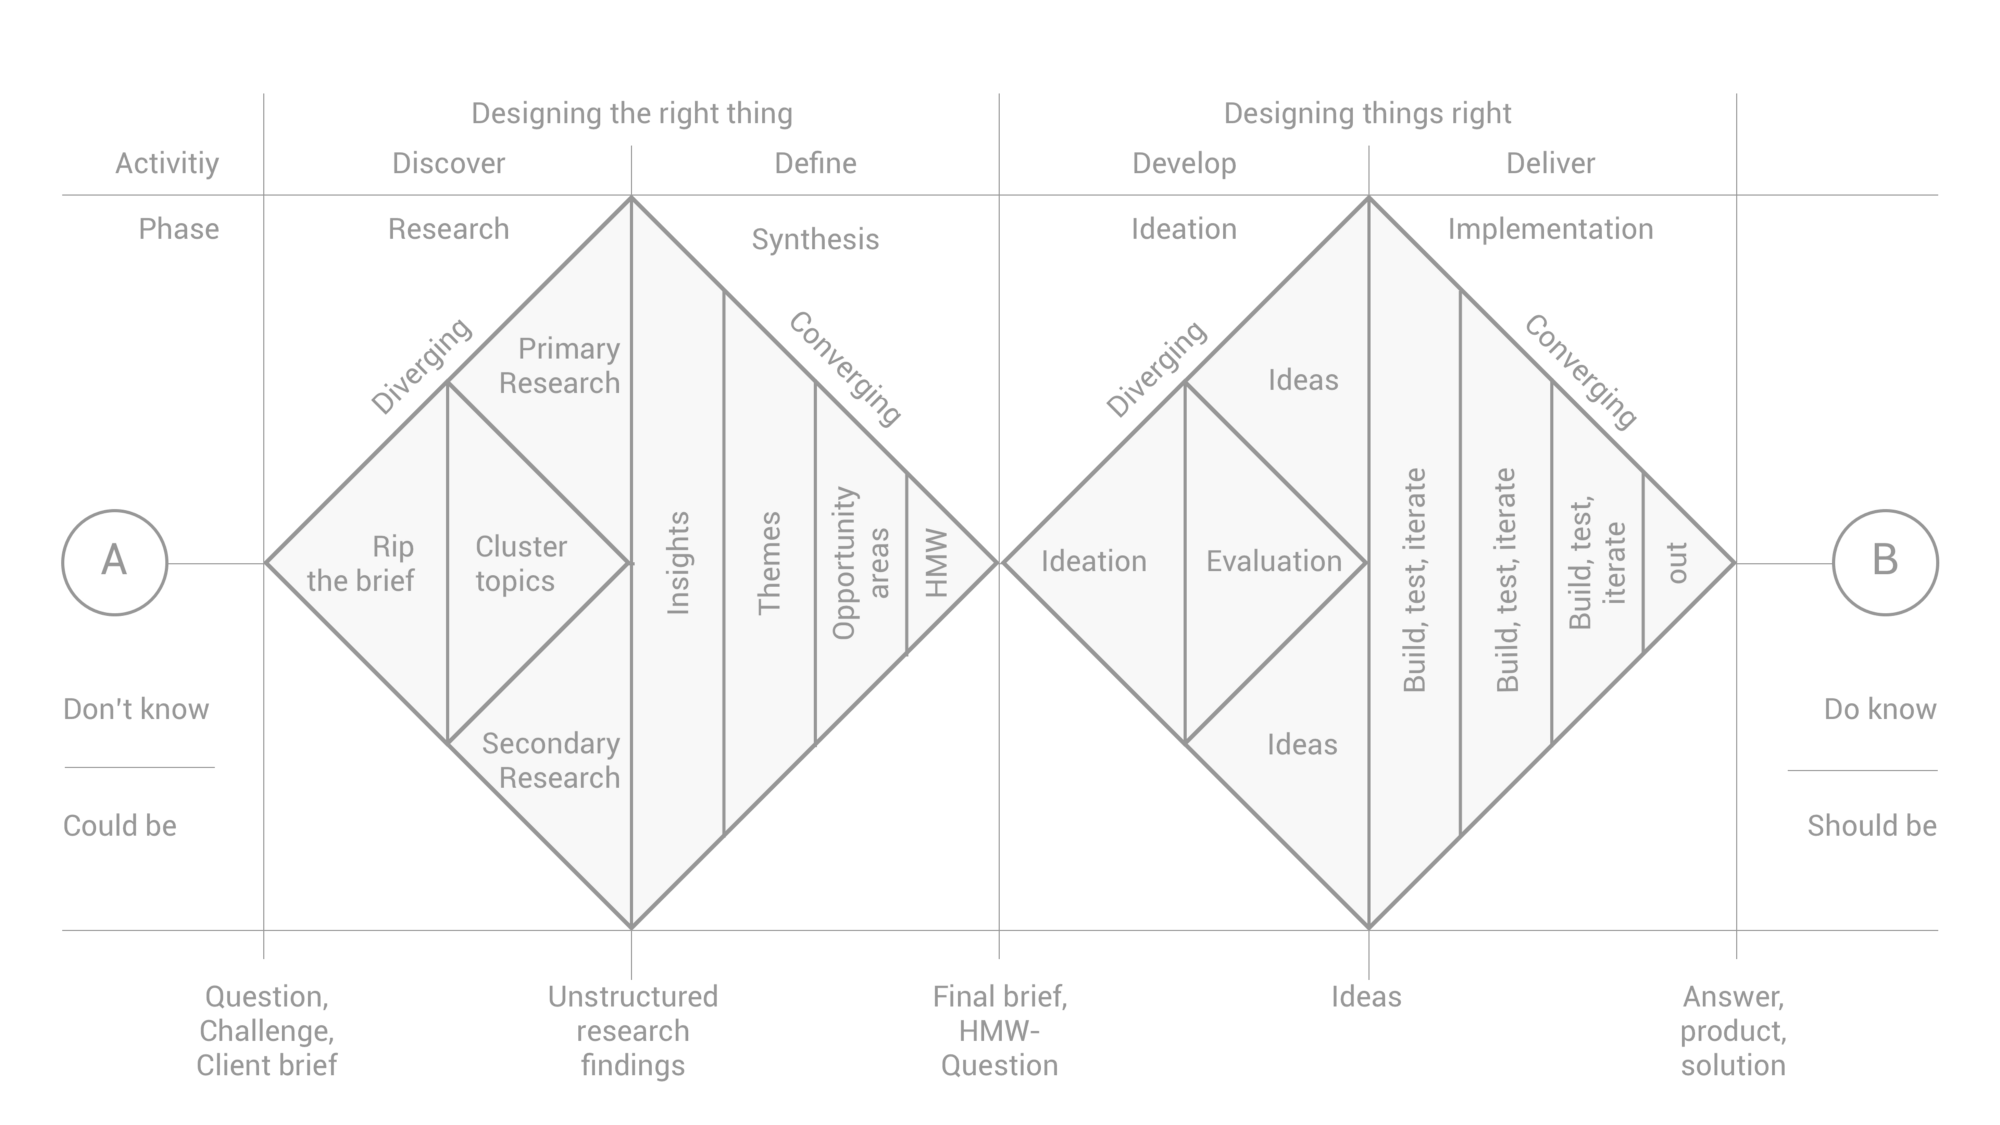
\includegraphics[width=\linewidth]{figures/summary/hcd-design-process}
	\caption{One version of the "Double Diamonds" to structure a traditional Human-Centered Design process. The P4P framework partially adapts this process and tailors it to password authentication. Image by Dan Nessler \url{https://medium.com/@dan.nessler} \la{24.03.2018}}
	\label{fig:summary:hcd-design-process}
\end{figure}

\subsubsection{Eight Recommendations for the Future}
% sanity check: who's the audience? % how far is this away from the research I've made?
The above summary allows us give recommendations on service design and research areas. Some bullets confirm prior work and listing them again should be seen as an emphasis. 
\begin{enumerate}
	% dynamic mental models
	\item \textbf{Consider the evolution of mental models}. Coping strategies adjust to the task load generated by passwords, which fluctuates throughout the years. Users might see complexity as the primary strength component, but this might change as service providers adjust to the recommendations from empirical usability research. 
	
	% strength is not all that important
	\item \textbf{Put less emphasis on password \textit{strength}}. Some researchers have demonstrated that beyond the threshold for online attacks, the benefits of increased password strength are limited. The most important scenarios that really require a strong (and usable!) password are master-passwords and accounts holding particularly sensitive data, e.g. a Dropbox that is full with health records or credit card details. 
	
	% more autonomy
	\item \textbf{Remove restrictions, give autonomy}. Service providers should eradicate unjustified complexity requirements, because they have strongly contributed to unreasonable mental models in the past. Instead, foster password diversity through autonomy, i.e. by empowering users to be creative and make informed decisions. We found that users want to be reasonably secure, but often lack the creativity to come up with adequate passwords.
	The \textit{show}-\textit{explain}-\textit{help}-\textit{empower} paradigm can overcome this creativity barrier and act as an overall guideline for authentication even beyond passwords.
	
	\item \textbf{Prepare for more requests of password replacement schemes}. More and more people are willing to use biometrics as primary authentication method\footurl{https://www-03.ibm.com/press/us/en/pressrelease/53646.wss}{26.03.2018}. They will expect this technology from products. However, companies often market biometrics as panacea for usable and secure authentication, and fail to make users aware of the ramifications. Therefore, passwords are going to be met with resistance and we need to reassure users that passwords have irrefutable benefits. 
		
	\item \textbf{Extend the method space}. We note a strong tendency towards studies facilitated through \gls{mTurk}. While the methodology is robust for eliciting quantitative data, the results are only one side of the truth. MTurk studies answer \textit{what works best}, but often fail to explain \textit{why} things work best. Therefore, resurrecting mixed-methods approaches that address qualitative aspects is recommendable for future USEC research. 
	
	\item \textbf{Stay realistic}. Nudges wear off over time, so we have to constantly create new persuasive strategies. Then again, users quickly resent paternalistic guidance and also prefer things to stay as they are. We have to acknowledge that there is only so much we can do. Persuasive support strategies will not work for all users in the same way, but if they reach even a small target group and make their lives a little easier, I believe that they are impactful enough. %Habituation has never really been a topic in password persuasion.
	
	\item \textbf{Follow risky ideas}. If we look at the current landscape of research on password support, the design space appears narrow: most published research tackles password meters in different facets. I argue that taking inspiration from other research areas, e.g. behavioral economics, can generate ideas outside the usual spectrum. They might be risky in terms of predictable effect size, but they certainly can counteract habituation effects. 
	% See section xyz. current support is somewhat gridlocked. we need more freshness. results with little to no significnant effects might not be easy to publish, but that's not a valid reason not to undertake the endeavor. 
	
	%\item \textbf{Leverage Trends}. % if biometric breaches become more prominent, it is time to ``sell'' passwords again. 
	
	\item \textbf{Give feedback}. Researchers mustn't expect that service providers read their papers. Point out where things go wrong. I've engaged in discussions with globally operating companies about their policies. This can generate real-world impact of millions of users instead of pushing h-indexes. I'm fairly sure only very few people will read this, so I intend to spread the word in other ways.
	
	%\item \textbf{Personalize user interfaces}. 
	%/ feedback etc. Hard challenge b/c user is not known at auth time. Browser APIs might help (Windows Auth API Hello). Password reset -- more info on user. % choice about authentication scheme --> older adults are more 
\end{enumerate}

\subsubsection{Conclusion}
This thesis has presented a new perspective on a well-known and perhaps unsolvable problem: coping with passwords is hard and annoying for most of us. Nonetheless, reducing the frustration component is a highly desirable goal. Hence, we contributed new insights into the factors that shape coping strategies (mental models, personality) and how to design for the users' implicit and explicit needs (a structured process to fine-tune the mixture of feedback, feedforward, and empowering technology). 

%Our findings can improve service design and guide future research. 

%The spectrum of problems is nuanced and solutions appear somehow gridlocked. We know much about the technical side and what people do to live with the password burden. What we do not know to its full extent is how exactly coping strategies form and how to support them best. What are the preconditions? Why do not all users behave the same way? How can we leverage that in designs? With the projects reported in this thesis, I aimed to tackle these aspects with ideas off the beaten path. Some of them came with a certain risk as to their feasibility and how to evaluate them. 

% How is PASDJO useful?
% How is the policy data set useful?
% How is the personality data useful?
% How is the Bubbles / Needs exploration useful?
% How is the emoji-passwords project useful? 
% How is the PWRM useful?
% Where do we go from here?

% so -- what did we learn? how has the world changed?
% you need to know the psychological aspects if you try to derive persuasive strategies. there's no way around it. 
% there are many solutions off the beaten path 
% very foundational, strategic, explorative character, risky research questions. 
% what does this mean for XYZ
% how does this change the world?
% thoughts. 


\section{Limitations}

\subsection{Generalizability}
% lab studies: mostly germans
% in the wild: also rather narrow geographic regions (Germany, UK, US)

\subsection{Study Designs}
% did the best we could, but there might have been other option
% not a


\subsection{Real-World Measurements}

\subsection{Nudging Ethics and Risks}




\section{Lessons Learned}
What would I do differently, if I had to do it all over again?



% KICKED OUT:

%\section{Classification and Dimensions}
%here we talk about in which way the projects contributed to the Framework? and in which way


% 
% not very different to the double diamond, but specificall tailored to password support systems.
% apply the process to demonstrate how design can be guided towards a real-solution.
% password manager.

% evlt noch weiter ausholen aus den bisherigen kapiteln was mitnehmen. 
%\section{Contributions} %TODO choose different name.
%give a walkthrough through all take-aways. that should do and create 1-2 pages. 
%
%\subsection{Theoretical Contributions}
%- framework for the design of password support strategies.
%
%\subsection{Methodological Contributions}
%- measuring passwords in the wild in an ethical way. (meta zxcvbn)
%- novel solution to measure password strength perception. (PASDJO)
%
%\subsection{Empirical Contributions}
%- the decoy effect and password suggestions
%- personality and passwords
%- mental models password managers
%
%\section{Implications}
%% how has this thesis advanced science? / the amount of the world's knowledge.
%\begin{itemize}
%\item Emoji authentication on the web - we're not there yet. 
%\end{itemize}

